\documentclass[french]{article}
\usepackage[T1]{fontenc}
\usepackage[utf8]{inputenc}
\usepackage{lmodern}
\usepackage[a4paper]{geometry}
\usepackage{babel}
\usepackage{graphicx}

\begin{document}
\title{Cahier des charges du Projet UNO}
\date{\today}
\author{Anthony Boens \\  Bilel Aloui \\  Alexis Verhaeghe}
\maketitle

\section{Définition du besoin}
\subsection{Contexte général}
Nous aimerions créer un jeu de cartes UNO en réseau de 4 joueurs. Le projet sera entièrement codé en C++. Nous utiliserons la librarie SFML pour les sockets et l'interface graphique. 

\subsection{Règles du jeu}
\subsubsection{But du jeu}
Le premier joueur qui n'a plus de cartes gagne la partie.

\subsubsection{Les cartes}
Il y a 108 cartes de 4 couleurs différentes (rouge, vert, jaune et bleu). Les cartes sont numérotées de 0 à 9 et ont chacune une couleur. Les cartes numérotées de 1 à 9 apparaissent 2 fois et le 0 une seule fois.
Il y a des 8 cartes \og  +2 \fg{} (2 de chaque couleur) qui ajoutent 2 cartes au joueur suivant, 8 cartes inversions (2 de chaque couleur) qui changent le sens du jeu et 8 cartes \og passe ton tour \fg{} (2 de chaque couleur) qui font passer le tour du joueur suivant.
Le paquet contient aussi 4 cartes \og  +4 \fg{} et \og joker \fg{} de couleur noire qui permettent de changer la couleur du jeu et d'ajouter 4 cartes au joueur suivant si c'est un \og +4 \fg{}.

\subsubsection{Déroulement du jeu}
Chaque joueur a 7 cartes et il y a une carte au hasard au milieu du tapis de jeu. Le joueur qui commence est désigné et doit jouer en fonction de cette carte.
On peut jouer une carte si elle est de la même couleur ou a le même chiffre que la carte sur le tapis. Si c'est une carte noire, on peut la jouer quand on veut et changer de couleur de jeu (le joueur suivant doit donc jouer en fonction de cette couleur).
Si le joueur ne peut pas jouer, il pioche une carte et si il ne peut toujours pas jouer, il passe son tour.
Si un joueur n'a plus qu'une carte, il doit dire \og UNO\fg{} pour avertir les autres adversaires.


\subsection{Besoins et priorités}
Le besoin principal du projet est d'avoir une partie entièrement fonctionnelle, qui gère toutes les cartes règlementaires dans le jeu UNO donc y compris les cartes bonus comme les +2, +4, passage de tour, changement de sens et les cartes joker.
L'autre besoin important et que la partie pourra se jouer en réseau avec les autres joueurs.

\section{Spécifications}
\begin{itemize}
	\item fonctionnalités de gestion des cartes
	\begin{itemize}
		\item gérer un paquet de 108 cartes
		\item distribution de 7 cartes aléatoires par joueurs
		\item gérer la pioche
		\item déterminer possibilité de jouer ou de passer
		\item afficher la carte courante (dernière carte jouée)
		\item gérer les cartes bonus
	\end{itemize}
	\item interface
		\begin{itemize}
			\item afficher les cartes du joueur
			\item interface graphique de résolution 1080x1920
			\item afficher le nombre de cartes des adversaires
			\item afficher texture de carte UNO
			\item afficher pioche et carte jouée carte
		\end{itemize}
	\item fonctionnalité
		\begin{itemize}
			\item afficher selecteur de 4 couleurs quand la carte \og changer de couleur\fg{} est jouée
			\item signe disctinctif du joueur courant
			\item affchier pop-up \og UNO \fg{} quand un joueur n'a qu'une seule
		\end{itemize}
	\item réseau
		\begin{itemize}
			\item gérer une partie serveur qui ditribue les cartes et applique les règles de jeux
			\item gérer une partie client qui voit les cartes et clique dessus pour jouer avec
		\end{itemize}
\end{itemize}

\section{Utilisation}

Pour jouer au jeu nous aurons 2 executables, un pour lancer le serveur et un autre pour le client.
On lance d'abord le serveur et ensuite le client. Le client se connectera automatiquement et à 4 joueurs la partie se lancera. Le serveur enverra une chaine de caractère du type \og 7b\fg{} pour la carte \og  7 bleu\fg{}. Nous distribuerons les cartes de cette façon. Pour jouer une carte, le client doit cliquer sur une carte et enverra une chaine de caractère du même type que nous avons vu. Avec cette chaine le serveur pourra mettre à jour l'interface graphique et les cartes du joueur.

\section{Livrable}
Le logiciel sera livré sur un dépot Github contenant le code source, un manuel d'installation et de configuration et un manuel d'utilisation.

\section{Diagramme de cas d'utilisation}
\begin{figure}
\centering
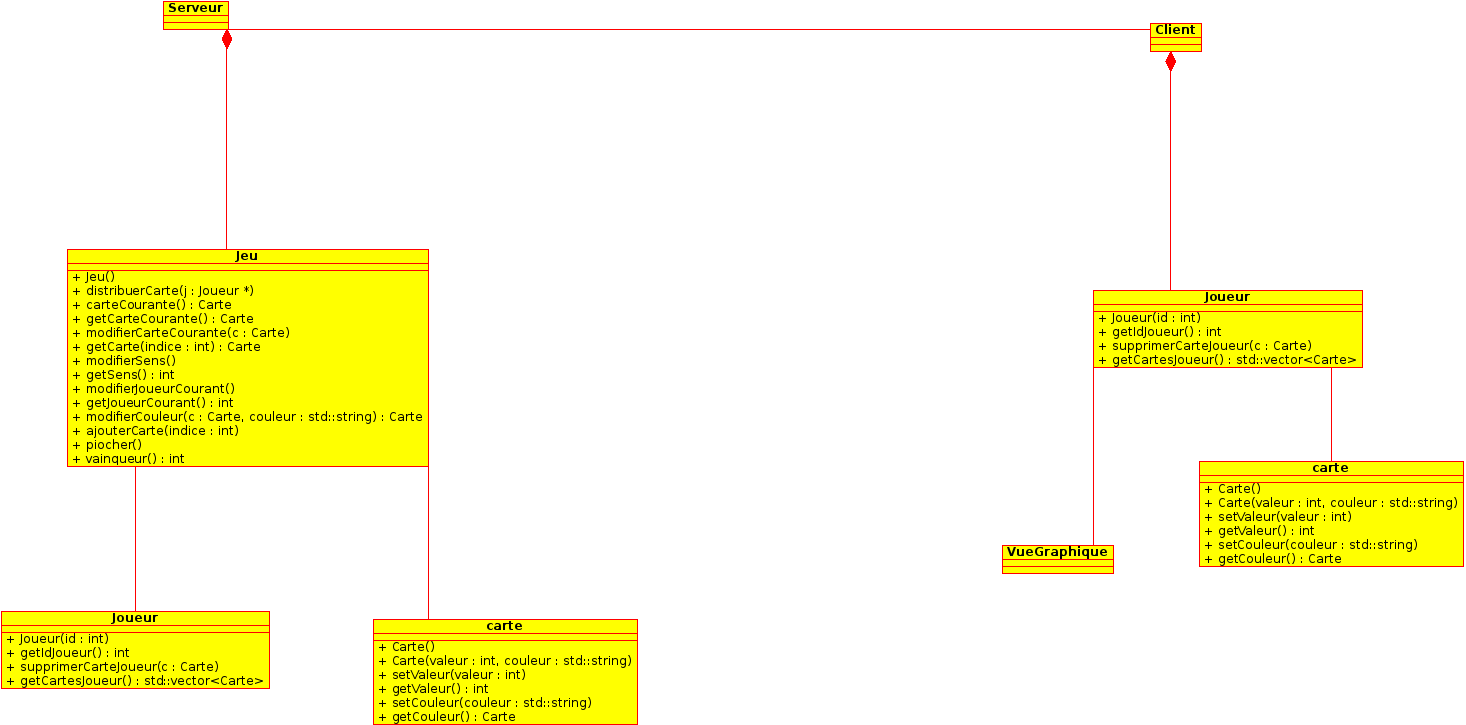
\includegraphics[width=0.7\linewidth]{class_diagram}
\caption{}
\label{classdiagram}
\end{figure}

Voir figure \ref{classdiagram}

\section{Maquette}
\begin{figure}
\centering
\includegraphics[width=0.7\linewidth]{"Screen maquette"}
\caption{}
\label{screen-maquette}
\end{figure}

Voir figure \ref{screen-maquette}


\end{document}
